\documentclass{beamer}
% Author: alick<alick9188@gmail.com>

% This file is modified from a solution template for:

% - Giving a talk on some subject.
% - The talk is between 15min and 45min long.
% - Style is ornate.

% Copyright 2004 by Till Tantau <tantau@users.sourceforge.net>.
%
% In principle, this file can be redistributed and/or modified under
% the terms of the GNU Public License, version 2.
%
% However, this file is supposed to be a template to be modified
% for your own needs. For this reason, if you use this file as a
% template and not specifically distribute it as part of a another
% package/program, I grant the extra permission to freely copy and
% modify this file as you see fit and even to delete this copyright
% notice.

\mode<presentation>
{
  \usetheme[secheader]{Boadilla}

  \setbeamercovered{transparent}
}

\usepackage{mflogo} % for \MF, \MP
\usepackage{graphicx}
\graphicspath{{fig/}}
\usepackage{listings}
\usepackage{xspace}
\usepackage{amsmath}
\usepackage{wasysym} % for \smiley etc
\usepackage{cclicenses} % CC symbols
\usepackage{fontspec}
\usepackage{xunicode,xltxtra}
\usepackage[CJKchecksingle]{xeCJK}

% xeCJK conf setup
\punctstyle{kaiming}
\renewcommand\CJKfamilydefault{\CJKsfdefault} % for slides

\setCJKmainfont[BoldFont={WenQuanYi Micro Hei},
ItalicFont={AR PL UKai CN}]{AR PL UMing CN}
\setCJKsansfont{WenQuanYi Micro Hei}
\setCJKmonofont+{WenQuanYi Micro Hei Mono}

\setCJKfamilyfont{zhsong}{AR PL UMing CN}
\setCJKfamilyfont{zhhei}{WenQuanYi Zen Hei}
\setCJKfamilyfont{zhkai}{AR PL UKai CN}

\newcommand*{\songti}{\CJKfamily{zhsong}} % 宋体
\newcommand*{\heiti}{\CJKfamily{zhhei}}   % 黑体
\newcommand*{\kaishu}{\CJKfamily{zhkai}}  % 楷书

\renewcommand\tablename{表格}

% fix: navi button not working with XeTeX
% SEE: http://bbs.ctex.org/viewthread.php?tid=64104
\makeatletter
\def\beamer@linkspace#1{%
  \begin{pgfpicture}{0pt}{-1.5pt}{#1}{5.5pt}
    \pgfsetfillopacity{0}
    \pgftext[x=0pt,y=-1.5pt]{.}
    \pgftext[x=#1,y=5.5pt]{.}
  \end{pgfpicture}}
\makeatother

\def\TeXLive{\TeX{} Live\xspace}
\let\TL=\TeXLive
% from btxdoc.tex
\def\BibTeX{{\rm B\kern-.05em{\sc i\kern-.025em b}\kern-.08em
    T\kern-.1667em\lower.7ex\hbox{E}\kern-.125emX}}

\title
{Fedora and \TL}

\author[alick] % (optional, use only with lots of authors)
{Zhao Tao\\ \texttt{alick9188@gmail.com}}

\institute[Thu] % (optional, but mostly needed)
{
  Department of Electronic Engineering\\
  Tsinghua University
}
% - Use the \inst command only if there are several affiliations.
% - Keep it simple, no one is interested in your street address.

\date[FAD Beijing 2011] % (optional)
{Oct 15, 2011 / FAD Beijing 2011}

\subject{Talks, TeX Live, FAD, Fedora}

% Delete this, if you do not want the table of contents to pop up at
% the beginning of each subsection:
\AtBeginSubsection[]
{
  \begin{frame}<beamer>{Outline}
    \tableofcontents[currentsection,currentsubsection]
  \end{frame}
}


% If you wish to uncover everything in a step-wise fashion, uncomment
% the following command:

%\beamerdefaultoverlayspecification{<+->}

\lstset{basicstyle=\ttfamily,breaklines=true}
\hypersetup{
%pdfpagemode=FullScreen,
}

\begin{document}

\begin{frame}
  \titlepage
\end{frame}

\begin{frame}{Outline}
  \tableofcontents
  % You might wish to add the option [pausesections]
\end{frame}


% Since this a solution template for a generic talk, very little can
% be said about how it should be structured. However, the talk length
% of between 15min and 45min and the theme suggest that you stick to
% the following rules:

% - Exactly two or three sections (other than the summary).
% - At *most* three subsections per section.
% - Talk about 30s to 2min per frame. So there should be between about
%   15 and 30 frames, all told.

\section{Introduction}

\subsection{\TeX}

\begin{frame}{What is \TeX ?}
  % - A title should summarize the slide in an understandable fashion
  %   for anyone how does not follow everything on the slide itself.

  \begin{itemize}
    \item a typysetting system for beautiful books
    \item originally developed by Donald E.~Knuth in 1978
    \item free to use, free to modify with naming exception
    \item \TeX\ 3.1415926 as of March 2008, and till today
  \end{itemize}
\end{frame}

\begin{frame}{Why \TeX\ (and why not)?}
  \begin{columns}[t]
    \begin{column}{.45\textwidth}
      \begin{block}{Pros}
        \begin{itemize}
          \item allow focusing on the content without bothering the
            layout(including TOC, references, etc)
          \item excel in typesetting math formular
            $$ \mathcal{F}(\xi)=\int_{-\infty}^{\infty}
            f(x)\mathrm{e}^{-\mathrm{j}2\pi \xi x}\,\mathrm{d}x $$
          \item enhanced in many aspects
            \begin{itemize}
              \item Chinese 華夏文明
              \item slides ({\scshape Beamer})
              \item music notes(\twonotes), chess, etc
            \end{itemize}
        \end{itemize}
      \end{block}
    \end{column}

    \begin{column}{.45\textwidth}
      \begin{block}{Cons}
        \begin{itemize}
          \item not WYSIWYG
          \item not easy to be \TeX{}pert
            \bigskip
          \item only .doc permitted
        \end{itemize}
      \end{block}
    \end{column}

  \end{columns}
\end{frame}

\begin{frame}{Overview}
  \begin{block}{\TeX\ system}
    \begin{itemize}
      \item Core: low-level macro language
      \item Formats: Plain \TeX, \alert{\LaTeX}, \AmS-\TeX, Con\TeX{}t
      \item Engines: tex, latex, pdf(la)tex, \alert{xe(la)tex}, lua(la)tex
      \item Distros: \TL, MiK\TeX, Mac\TeX
    \end{itemize}
  \end{block}
\end{frame}

\subsection{\TeXLive}

\begin{frame}{What is \TL ?}
  \begin{itemize}
    \item a \TeX\ distro: a comprehensive collection of \TeX\ utils

      Schemes
      \begin{itemize}
        \item Collections
          \begin{itemize}
            \item Packages
          \end{itemize}
      \end{itemize}

    \item developed since 1996 by TeX user groups
    \item originally for Linux, now cross-platform
    \item can run live from a DVD (up to v2009)
  \end{itemize}
\end{frame}

\section{Install \TL}
\subsection{local version}
\begin{frame}{Methods}
  \begin{description}
    \item[\frownie] download the huge DVD iso
      \pause
    \item[\$\$] be a member of TUG and get \TL on DVD
      \pause
    \item[\smiley] net install
  \end{description}
\end{frame}

\begin{frame}[fragile]
  \frametitle{网络安装}
  \begin{itemize}
    \item
从 CTAN 镜像下载
install-tl-unx.tar.gz
和
install-tl-unx.tar.gz.sha256
\begin{itemize} % several mirror url
  \item \url{http://mirrors.tuna.tsinghua.edu.cn/CTAN/systems/texlive/tlnet/}
  \item \url{http://ftp.ctex.org/mirrors/CTAN/systems/texlive/tlnet/}
  \item More at \url{http://mirror.ctan.org/README.mirrors}
\end{itemize}

\item 校验
\begin{lstlisting}
$ LANG=C sha256sum --check install-tl-unx.tar.gz.sha256
install-tl-unx.tar.gz: OK
\end{lstlisting}

  \end{itemize}
\end{frame}

\begin{frame}[fragile]
  \frametitle{网络安装}
  \begin{itemize}
    \item Install 安装
      \begin{lstlisting}
su -c'./install-tl -gui -repository http://mirrors.tuna.tsinghua.edu.cn/CTAN/systems/texlive/tlnet/'
      \end{lstlisting}

      \begin{itemize}
        \item 图形安装界面需要 Perl Tk 模块:\texttt{yum install
          perl-Tk}
        \item root 使用 X 程序,可能还需要 \texttt{xhost
          +si:localuser:root}
      \end{itemize}
\item 截图\dots
\end{itemize}
\end{frame}

\begin{frame}
  \begin{figure}[h]
  \centering
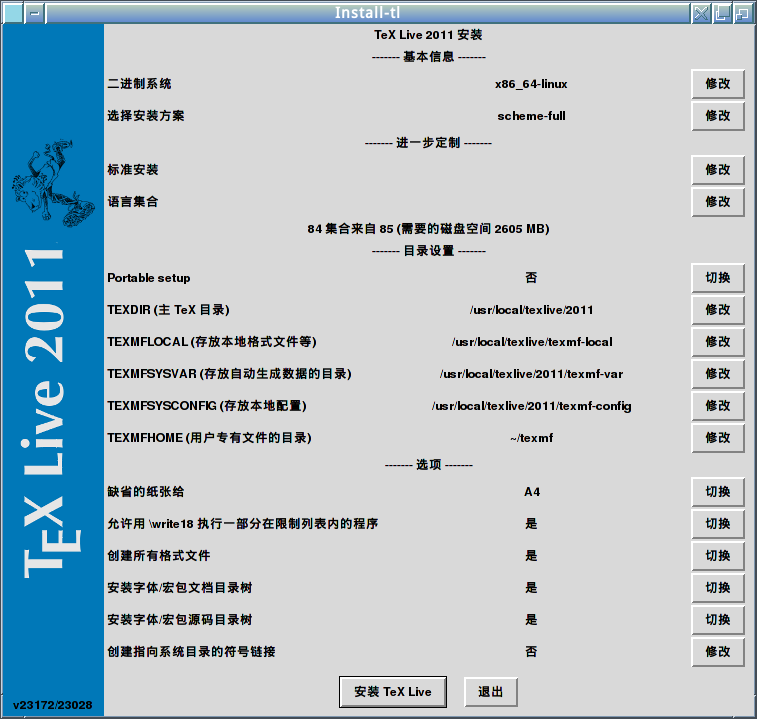
\includegraphics[scale=0.35]{main-init.png}
  \end{figure}
\end{frame}

\begin{frame}
  \begin{figure}[h]
  \centering
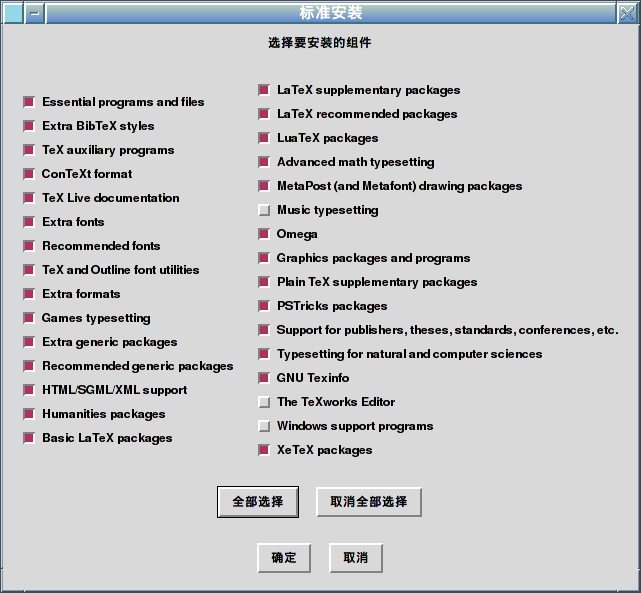
\includegraphics[scale=0.4]{标准安装.png}
  \end{figure}
\end{frame}

\begin{frame}
  \begin{figure}[h]
  \centering
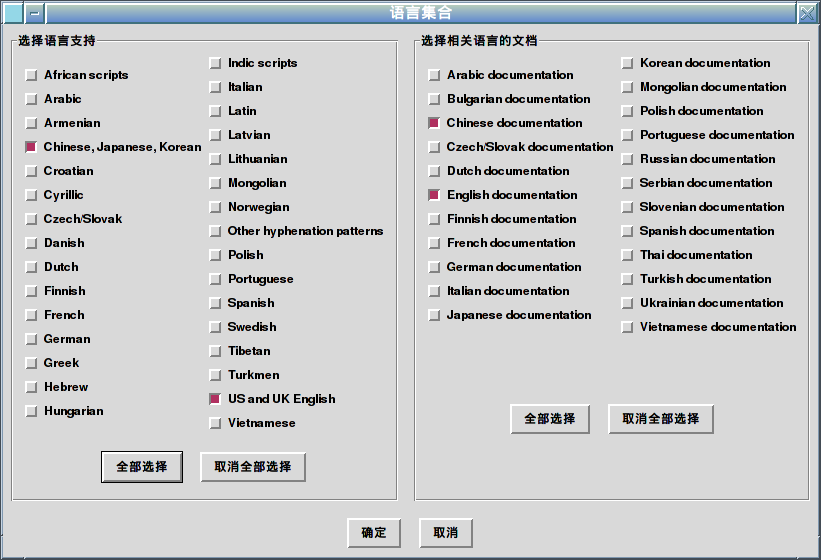
\includegraphics[scale=0.4]{语言集合.png}
  \end{figure}
\end{frame}

\begin{frame}
  \begin{figure}[h]
  \centering
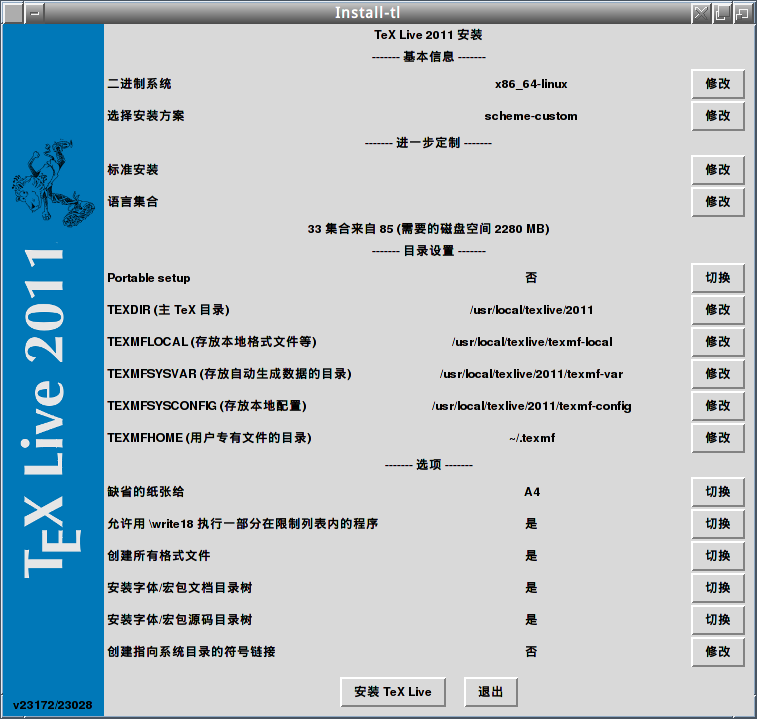
\includegraphics[scale=0.35]{main-customed.png}
  \end{figure}
\end{frame}

% 安装进行中
\begin{frame}
  \begin{figure}[h]
  \centering
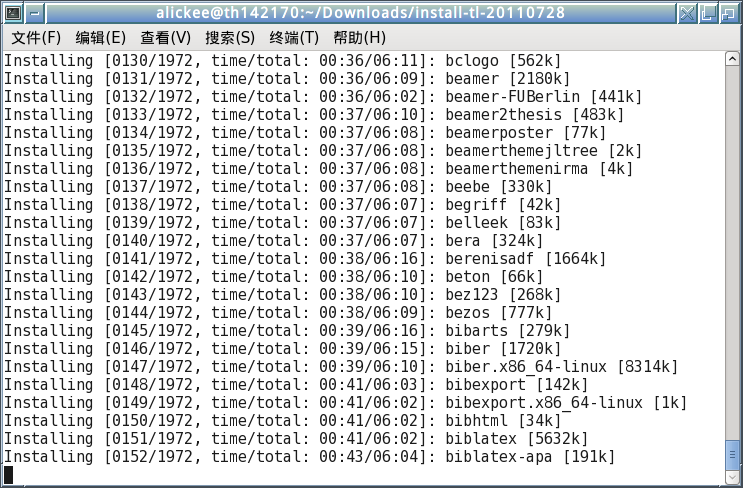
\includegraphics[scale=0.45]{term.png}
  \end{figure}
\end{frame}

% 安装完成
\begin{frame}
  \begin{figure}[h]
  \centering
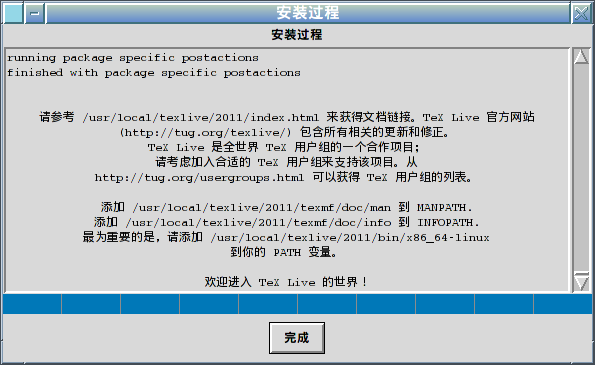
\includegraphics[scale=0.5]{安装过程.png}
  \end{figure}
\end{frame}

\begin{frame}[fragile]
  \frametitle{网络安装后配置}
\begin{itemize}
  \item
    Add the following lines into your \nolinkurl{~/.bash_profile}:
    \begin{lstlisting}
export PATH=/usr/local/texlive/2011/bin/x86_64-linux:$PATH
export MANPATH=/usr/local/texlive/2011/texmf/doc/man:$MANPATH
export INFOPATH=/usr/local/texlive/2011/texmf/doc/info:$INFOPATH
    \end{lstlisting}

  \item
打开 \TeXLive 指南中文版 ``texlive-zh-cn.pdf'',
关注第 3.4 节
  \begin{lstlisting}
texdoc texlive-zh
  \end{lstlisting}

\end{itemize}
\end{frame}

\begin{frame}[fragile]
  \frametitle{网络安装后配置}
  \begin{itemize}
\item
\XeTeX\ and fontconfig:
\begin{lstlisting}
cp /usr/local/texlive/2011/texmf-var/fonts/conf/texlive-fontconfig.conf /etc/fonts/conf.d/09-texlive.conf
fc-cache -fsv
\end{lstlisting}

\item Con\TeX{}t Mark IV
  \begin{lstlisting}
context --generate
  \end{lstlisting}

\end{itemize}
\end{frame}

\lstdefinestyle{latex}{
language={[LaTeX]TeX},
frame=single,
escapeinside=``,
keywordstyle=\color{red!70},
}

\begin{frame}
  \frametitle{网络安装后测试}
  \framesubtitle{English Tests}

  \begin{exampleblock}{Use installed sample files:}
    \begin{itemize}
      \item \texttt{latex sample2e.tex \#} .tex $\rightarrow$ .dvi (device independent)

      \texttt{xdvi sample2e.dvi \#} also try dvipdf sample2e.dvi
      \item try \texttt{pdflatex sample2e} directly
      \item \texttt{xetex opentype-info.tex \#} test of xetex's OpenType support
    \end{itemize}

  \end{exampleblock}
\end{frame}

\begin{frame}[fragile]
  \frametitle{网络安装后测试}
  \framesubtitle{中文测试 ``test-chinese.tex''}
  \begin{columns}[t]
    \begin{column}{.45\textwidth}
\begin{lstlisting}[style=latex]
\documentclass{ctexart}
\setCJKmainfont{AR PL UMing CN}
\begin{document}
\TeX{}`你好!`
\end{document}
\end{lstlisting}
\end{column}
    \begin{column}{.45\textwidth}
  \begin{lstlisting}
xelatex test-chinese
evince test-chinese.pdf
  \end{lstlisting}
  \fbox{\textrm \TeX{}\songti 你好!}
\end{column}
\end{columns}

\end{frame}

\subsection{sys version/ rpm}

% TeX Live in Linux distro repo
% Ubuntu: as of July 2011 the texlive package that ships with Ubuntu
% (TeX Live 2009) is lagging two years behind the current TeX Live
% release (TeX Live 2011). (https://help.ubuntu.com/community/LaTeX)

\begin{frame}
  \begin{table}[htbp]
	\centering
	\caption{调查结果}
	\begin{tabular}{lllp{6em}}
		\hline
版本		&仓库	&安装方式/发行版&体验\\
		\hline
2011		&CTAN	&ISO(BT)	&强大 \\
2011		&distro	&Gentoo Portage	&少许问题 \\
2011		&CTAN	&net		&Debian sid 刚用不久 \\
2010,2011	&?	&?		&Debian 很好 \\
2010		&CTAN	&net		&XP+Linux 挺好除了不能滚动升级 \\
2007		&distro	&Fedora 15	&xetex 挺好 \\
2009		&distro	&Ubuntu 10.04	&已有xecjk \\
2011		&CTAN	&net		&不错 \\
2009		&distro	&Ubuntu 11.04	&xelatex \\
		\hline
	\end{tabular}
	\label{tab:poll_result}
\end{table}


\end{frame}

\begin{frame}
  \frametitle{\TL in Linux distros}
  \begin{itemize}
    \item Fedora offical repo: \TL 2007 \hfill Not good.
    \item Ubuntu offical repo: \TL 2009 \hfill Not good.
    \item jnovy's repo \TL 2010\&2011 \hfill \alert{Good} news.

      \url{http://fedoraproject.org/wiki/Features/TeXLive}
  \end{itemize}
\end{frame}

% jnovy's repo 2011
\begin{frame}[fragile]
  \frametitle{安装步骤}

\begin{lstlisting}
rpm -i http://jnovy.fedorapeople.org/texlive/packages.f14/texlive-release.noarch.rpm
yum clean all
yum install texlive # basic scheme
OR yum install texlive-scheme-full # if disk space is enough
\end{lstlisting}

\begin{lstlisting}
yum install texlive-collection-xetex texlive-ctex
yum install 'tex(savesym.sty)'
yum install 'tex(siunitx.sty)'
\end{lstlisting}

\begin{lstlisting}
xelatex template-xetex.tex
\end{lstlisting}

\end{frame}

\begin{frame}{Why rpm?}
  \begin{itemize}
    \item single installation tool
    \item package dependency
    \item no old packages in \TL repo
  \end{itemize}
  \vskip0pt plus.5fill
  \begin{itemize}
    \item Volunteers needed
  \end{itemize}
\end{frame}

\section{Use \TL}

\subsection{Tips}
\begin{frame}{General Tips}
  \begin{itemize}
    \item focus on the content, not the layout
      \begin{itemize}
        \item use well-defined classes/templates: ctexart, beamer,
          thuthesis
        \item packages: siunitx, listings, xeCJK
        \item structure: section, subsection, etc
        \item meaning: emph, label
      \end{itemize}
    \item \texttt{texcount -ch report.tex}: count words
    \item Project(input, include, Makefile, git)
    \item Which TeX Editor? (Vim, Emacs, LyX, TeX IDE\dots)
  \end{itemize}
\end{frame}

\subsection{Get Help}
\begin{frame}{Help Yourself}
  \begin{itemize}
    \item tlmgr (Yum in Fedora version)
      \begin{itemize}
        \item \texttt{tlmgr gui}
        \item \texttt{man tlmgr}
      \end{itemize}

    \item texdoc (may need yum install)
      \begin{itemize}
        \item e.g. \texttt{texdoc xecjk},
          \texttt{texdoc mathmode}, and \texttt{texdoc symbols}
        \item \texttt{texdoctk} --- GUI
      \end{itemize}
  \end{itemize}
\end{frame}

\begin{frame}{\TeX\ community}
  \begin{columns}[c]
    \begin{column}{.45\textwidth}
      \begin{itemize}
        \item BBS
          \begin{itemize}
            \item \href{http://www.newsmth.net/nForum/board/TeX}{smth TeX
              board}
            \item \href{http://bbs.ctex.org/}{bbs.ctex.org}
          \end{itemize}
        \item Mailing list
          \begin{itemize}
            \item \href{http://tug.org/mailman/listinfo/tex-live}{\TL}
            \item \href{http://www.linux.cz/pipermail/texlive/}{Fedora \TL
              Packaging}
          \end{itemize}
        \item \href{http://www.tex.ac.uk/cgi-bin/texfaq2html}{UK FAQ}
        \item \href{http://justfuckinggoogleit.com/}{Google}
      \end{itemize}
    \end{column}
    \begin{column}{.45\textwidth}
      
\includegraphics[width=\textwidth]{TFZsuperellipse-crop.pdf}
    \end{column}
  \end{columns}
\end{frame}

\section*{Summary}

\begin{frame}{Summary}

  % Keep the summary *very short*.
  \begin{itemize}
  \item \TL makes typesetting easy.
  \item The installation of \TL is easy.
  \item Happy \LaTeX{}ing!
  \end{itemize}

  % The following outlook is optional.
  \vskip0pt plus.5fill
  \begin{itemize}
  \item
    Outlook
    \begin{itemize}
      \item \textit{MakeIndex}, \BibTeX
    \item \MP, Asymptote
    \end{itemize}
  \end{itemize}
\end{frame}

\section*{Auxiliary}

\begin{frame}
  \begin{itemize}
    \item Get these materials from \alert{github}
      \begin{itemize}
        \item templates: \url{http://github.com/alick9188/TeXLab}
        \item FAD slides: \url{http://github.com/alick9188/fad-texlive-talk}
      \end{itemize}
    \item License: CC BY-SA 3.0 Unported \cc\ccby\ccsa
  \end{itemize}
\end{frame}

\begin{frame}
  \begin{center}
    {\LARGE Thanks!
    \bigskip

    Questions?}

  \end{center}
\end{frame}

\end{document}
%%% vim: set sw=2 isk+=\: et tw=70 formatoptions+=mM:
